\section{Experiments}
\label{sec:experiments}

\draftnote{Populate from the formal evaluation manifest, not the obsolete
six-task matrix. Report every task by source and protocol.}

\subsection{Research Questions}

\begin{description}
    \item[RQ1: Generality.] Can one model remain competitive across correctness,
    response, misconception, and prospective-behavior tasks?
    \item[RQ2: Capability.] Can the model generate concrete responses, natural-
    language misconception diagnoses with evidence, prospective behavior, and
    persistence judgments that correctness-only KT does not natively expose?
    \item[RQ3: Transfer.] Does training on one educational task or supervision
    type improve a distinct held-out educational task under exposure-matched
    controls, including but not limited to synthetic-to-real diagnosis?
    \item[RQ4: State validity.] Does a frozen history-closed State8 predict and
    explain future behavior for unseen students, does pairing the state with
    its owner's outcomes matter, and are predictions stable across disjoint
    views of the same observed history?
\end{description}

\subsection{Datasets and Protocols}

\draftnote{Add the 259,845-example training table and 21,676-example formal
evaluation table, then separate T1, T2-choice, T2-open, T3-taxonomy,
T3-generation, T4 by prediction distance, and strict T5. Report T6
future-KC-performance only in the appendix.}

\subsection{Baselines and Metrics}

\draftnote{Describe IRT, PFA, BKT, DKT, AKT, conditional response models,
full-taxonomy retrieval, and persistence logistic regression. Do not compare
LLM-judge semantic accuracy and exact taxonomy accuracy as if identical.}

\subsection{Main Results}

\draftnote{Insert multi-seed results and confidence intervals. Current formal
matrix is suitable as a preliminary run, not a final ICLR table.}

\subsection{Method Ablations}

We compare: (i)~the unrestricted full-context model; (ii)~the existing
one-shot late-fusion bottleneck; (iii)~the recurrent architecture with only
$\mathcal L_{\mathrm{gen}}$; (iv)~variants removing distillation, trajectory
consistency, or counterfactual grounding; and (v)~the complete \model.  The
primary method diagnostic is the state-compression gap between the frozen
full-context teacher and the state-only decoder on identical examples.  We
also report accuracy or generation quality as a function of history length and
number of recurrent updates.

\subsection{Transfer and Student-State Analyses}

\draftnote{Add exposure-matched C3 ablations; State8 versus population and
same-window baselines; state-ownership permutation tests; disjoint-history
stability; readable future profiles; recurrent state drift; and one-shot
versus recurrent state comparisons.  Report literal donor, same-profile,
random, and no-op swaps as diagnostics rather than C4 gates.}

\subsection{Controlled Evidence for a One-Shot Causal State}
\label{sec:c4-one-shot}

We separately audit the strongest completed one-shot bottleneck, without
using it as evidence for recurrent closure.  On each frozen intervention pair,
the native recipient prediction is the recipient-rule response $B$.  We then
replace the residual stream at the single state-token address with either the
matched donor trajectory, norm-matched Gaussian residual noise, a same-rule
donor trajectory, or the recipient's own trajectory (no-op).  The primary
contrast is
\begin{equation}
    D_{\mathrm{specific}}
    = \Pr(\widehat r=r_A\mid\text{directed donor})
    - \Pr(\widehat r=r_A\mid\text{Gaussian noise}),
\end{equation}
computed only on pairs for which the native model predicts $B$.  Here
``random'' is deliberately an out-of-distribution Gaussian-noise control, not
a randomly selected student's state.

\begin{figure}[t]
    \centering
    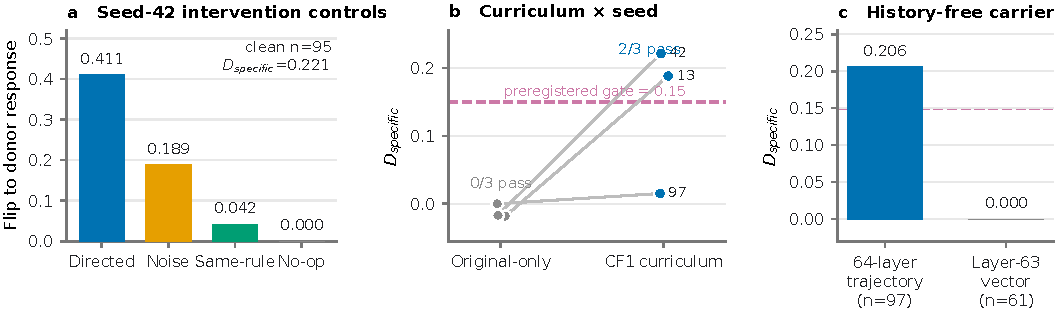
\includegraphics[width=\linewidth]{figures/c4_causal_state.pdf}
    \caption{\textbf{A causally specific one-shot student-state route is
    conditional on training and is carried across depth.}
    \captiona\ On the canonical CF1 + vision-pad seed-42 checkpoint, replacing
    the state-token trajectory with a matched donor trajectory changes the
    recipient prediction to the donor response in $0.411$ of the clean pairs,
    versus $0.189$ for norm-matched Gaussian noise, $0.042$ for a same-rule
    donor, and $0.000$ for no-op ($n=95$; $D_{\mathrm{specific}}=0.221$).
    \captionb\ The preregistered threshold $D_{\mathrm{specific}}\geq0.15$ is
    met by two of three historical CF1 runs but by none of the original-only
    runs; all seed-level results remain visible.  Thus the counterfactual
    curriculum is necessary in this factorial but is not sufficient across
    optimization runs.  The historical trainer did not seed model and LoRA
    construction before module initialization, so these are run-level rather
    than fully controlled training-seed replications.
    \captionc\ In a strict zero-training bridge, the decoder receives no raw
    history and has no persistent history KV cache.  Transferring the same
    address across all 64 residual layers preserves causal specificity
    ($D_{\mathrm{specific}}=0.206$, $n=97$), whereas transferring only its
    final layer-63 vector causes no prediction changes
    ($D_{\mathrm{specific}}=0$, $n=61$).  The completed evidence therefore
    supports a one-address, depth-indexed residual trajectory, not a compact
    final-layer vector or recurrent/Markov state.}
    \label{fig:c4-causal-state}
\end{figure}
